\subsection{Drude model, Ohm's Law and Kinetic Inductance}

\begin{frame}{Drude model, Ohm's Law and Kinetic Inductance}

\begin{columns}
    \column{0.55\textwidth}
    Electronic equation of motion:
    \begin{equation*}
        \dfrac{d}{dt} \langle m \mathbf{v}(t) \rangle = e \mathbf{E} - \dfrac{ \langle m \mathbf{v}(t) \rangle}{\tau}.
    \end{equation*}
    where \( \tau \sim 10^{-14} \si{s} \) is a constant. \\
    Equivalent circuit:
    \begin{equation*}
        R = \dfrac{m}{N e^2 \tau} \dfrac{l}{S}, \ \ L_K = \dfrac{m}{N e^2} \dfrac{l}{S}.
    \end{equation*}
    where the current: \( i = N e v S\), \\
    Number density of free electrons: \(N\).

    \begin{itemize}
        \item \( L_K \rightarrow 0\): Ohm's Law.
        \item \( L_K \neq 0\): High frequency, Superconductor.
    \end{itemize}
    
    \column{0.45\textwidth}
    \vspace{-8mm}
    \begin{figure}[!htb]
        \centering
        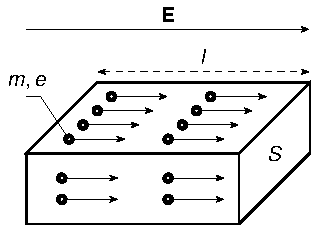
\includegraphics[width=\textwidth]{Figures/Electrons_in_Drude_model.pdf}
        \caption{Electrons in Drude model.}
        \label{Drude_model}
    \end{figure}
    \vspace{-6mm}
    \begin{figure}[!htb]
        \centering
        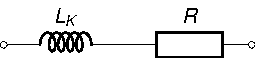
\includegraphics[width=0.9\textwidth]{Figures/Equivalent_circuit_of_Drude_model.pdf}
        \caption{Equivalent circuit of Drude model.}
        \label{Equivalent_circuit_of_Drude_model}
    \end{figure}
    
\end{columns}
    
\end{frame}